%%%%%%%%%%%%%%%%%%%%%%%%%%%%%%%%%%%%

\section{二項分布}

%%%%%%%%%%%%%%%%%%%%%%%%%%%%%%%%%%%%

\subsection{二項分布}

%%%%%%%%%%%%%%%%%%%%%%%%%%%%%%%%%%%%

\begin{frame}[shrink=25]

\dq{実験に参加するために4人を無作為に選んだとする。そのうちちょうど1人がショックを与えることを拒否する確率は何か？}

これらの人をアレン（A）、ブリタニー（B）、キャロライン（C）、デイミアン（D）と呼ぼう。以下の4つのシナリオそれぞれが「ちょうど1人が拒否する」という条件を満たす：\\
\vspace{0.25cm}
\begin{changemargin}{+1.5cm}{+0cm}
{\footnotesize
\begin{enumerate}
\item[シナリオ1:] $\slot{0.35}{\text{(A) \orange{拒否}}} \times \slot{0.65}{\text{(B) ショック}} \times \slot{0.65}{\text{(C) ショック}} \times \slot{0.65}{\text{(D) ショック}} = 0.0961$
\item[シナリオ2:] $\slot{0.65}{\text{(A) ショック}} \times \slot{0.35}{\text{(B) \orange{拒否}}}\times \slot{0.65}{\text{(C) ショック}} \times \slot{0.65}{\text{(D) ショック}} = 0.0961$
\item[シナリオ3:] $\slot{0.65}{\text{(A) ショック}} \times \slot{0.65}{\text{(B) ショック}} \times \slot{0.35}{\text{(C) \orange{拒否}}}\times \slot{0.65}{\text{(D) ショック}} = 0.0961$
\item[シナリオ4:] $\slot{0.65}{\text{(A) ショック}} \times \slot{0.65}{\text{(B) ショック}} \times \slot{0.65}{\text{(C) ショック}} \times \slot{0.35}{\text{(D) \orange{拒否}}} = 0.0961$
\end{enumerate}
}
\end{changemargin}
4人のうちちょうど1人がショックを与えることを拒否する確率は、これらすべての確率の和である。
\[ 0.0961+ 0.0961 + 0.0961 + 0.0961 = 4 \times 0.0961 = 0.3844 \]

\end{frame}

%%%%%%%%%%%%%%%%%%%%%%%%%%%%%%%%%%%%

\begin{frame}
\frametitle{二項分布}

前のスライドの問いは、$n$ 回の試行中の成功回数 \mathhl{k} の確率（$n = 4$ 回中 $k = 1$ 回の成功）を求めており、この確率を次のように計算した
\[ \text{シナリオ数} \times P(\text{1つのシナリオ}) \]

\begin{itemize}

\item $\text{シナリオ数}$：これを計算するより簡単な方法がある。後ほど説明する……

\item $P(\text{1つのシナリオ}) = p^k~(1-p)^{(n-k)}$ \\
{\tiny 成功確率の成功回数乗、失敗確率の失敗回数乗}

\end{itemize}

\hl{二項分布}は、成功確率 $p$ の $n$ 回の独立なベルヌーイ試行においてちょうど $k$ 回成功する確率を記述する。

\end{frame}

%%%%%%%%%%%%%%%%%%%%%%%%%%%%%%%%%%%%

\begin{frame}
\frametitle{シナリオ数の数え方}

先ほど、ちょうど1人がショックを与えることを拒否するという条件に合うすべてのシナリオを書き出した。もし $n$ がより大きく、$k$ が1以外の場合、例えば $n = 9$、$k = 2$ では：

\begin{center}
\begin{tabular}{c}
\orange{R}\orange{R}SSSSSSS \\
S\orange{R}\orange{R}SSSSSS \\
SS\orange{R}\orange{R}SSSSS \\
$\cdots$ \\
SS\orange{R}SS\orange{R}SSS \\
$\cdots$ \\
SSSSSSS\orange{R}\orange{R} \\
\end{tabular}
\end{center}

すべてのシナリオを書き出すことは非常に面倒で誤りが起きやすい。

\end{frame}

%%%%%%%%%%%%%%%%%%%%%%%%%%%%%%%%%%%%

\begin{frame}[fragile]
\frametitle{シナリオ数の計算}

\formula{二項係数}
{
\hl{二項係数}（choose 関数）は、$n$ 回の試行で $k$ 回成功する方法の数を計算するのに役立つ。
\[ {n \choose k} = \frac{n!}{k! (n - k)!} \]
}

\begin{itemize}

\item $k = 1$、$n = 4$：${4 \choose 1} = \frac{4!}{1! (4 - 1)!} = \frac{4 \times 3 \times 2 \times 1}{1 \times (3 \times 2 \times 1)} = 4$

\item $k = 2$、$n = 9$：${9 \choose 2} = \frac{9!}{2! (9 - 2)!} = \frac{9 \times 8 \times 7!}{2 \times 1 \times 7!} = \frac{72}{2} = 36$

\end{itemize}

\vfill

\Note{R を使っても計算できる：}
\begin{beamerboxesrounded}[shadow = true, lower = code body]{}
{\small
\begin{verbatim}
> choose(9,2)
[1] 36
\end{verbatim}
}
\end{beamerboxesrounded}

\end{frame}

%%%%%%%%%%%%%%%%%%%%%%%%%%%%%%%%%%%

\begin{frame}[fragile]
\frametitle{二項係数の性質}

\pq{次のうち誤りはどれか？}

\begin{enumerate}[(a)]
\item $n$ 回の試行で1回成功する方法は $n$ 通りある、${n \choose 1} = n$。
\item $n$ 回の試行で $n$ 回成功する方法は1通りしかない、${n \choose n} = 1$。
\item $n$ 回の試行で $n$ 回失敗する方法は1通りしかない、${n \choose 0} = 1$。
\solnMult{$n$ 回の試行で $n-1$ 回成功する方法は $n-1$ 通りある、${n \choose n-1} = n-1$。}
\end{enumerate}

\end{frame}

%%%%%%%%%%%%%%%%%%%%%%%%%%%%%%%%%%%

\begin{frame}
\frametitle{二項分布（続き）}

\formula{二項確率}
{
$p$ が成功確率、$(1-p)$ が失敗確率、$n$ が独立試行回数、$k$ が成功回数を表すとき
\[P(n\text{回中}~k\text{回の成功}) = {n \choose k}~p^k~(1-p)^{(n-k)} \]
}


\end{frame}

%%%%%%%%%%%%%%%%%%%%%%%%%%%%%%%%%%%

\begin{frame}

\pq{二項分布を適用するために満たす必要のない条件はどれか？}

\begin{enumerate}[(a)]
\item 試行は独立でなければならない
\item 試行回数 $n$ は固定されていなければならない
\item 各試行の結果は\textit{成功}または\textit{失敗}に分類されなければならない
\solnMult{望ましい成功回数 $k$ は試行回数より大きくなければならない}
\item 成功確率 $p$ は各試行で同じでなければならない
\end{enumerate}

\end{frame}

%%%%%%%%%%%%%%%%%%%%%%%%%%%%%%%%%%%

\begin{frame}
\frametitle{}

\pq{2012年のギャラップ調査によると、アメリカ人の26.2\%が肥満である。10人のアメリカ人の無作為標本の中で、ちょうど8人が肥満である確率は何か？}

\begin{enumerate}[(a)]
\item かなり高い
\solnMult{かなり低い}
\end{enumerate}

\vfill

\ct{Gallup: \webURL{http://www.gallup.com/poll/160061/obesity-rate-stable-2012.aspx}, January 23, 2013.}

\end{frame}

%%%%%%%%%%%%%%%%%%%%%%%%%%%%%%%%%%%%

\begin{frame}

\pq{2012年のギャラップ調査によると、アメリカ人の26.2\%が肥満である。10人のアメリカ人の無作為標本の中で、ちょうど8人が肥満である確率は何か？}

\begin{enumerate}[(a)]
\item $0.262^8 \times 0.738^2$
\item ${8 \choose 10} \times 0.262^8 \times 0.738^2$
\solnMult{${10 \choose 8} \times 0.262^8 \times 0.738^2$} \only<2->{\orange{$ = 45 \times  0.262^8 \times 0.738^2 = 0.0005$}}
\item ${10 \choose 8} \times 0.262^2 \times 0.738^8$
\end{enumerate}



\end{frame}

%%%%%%%%%%%%%%%%%%%%%%%%%%%%%%%%%%%

\begin{frame}
\frametitle{誕生日問題}

\dq{無作為に選んだ2人が同じ誕生日を持つ確率は何か？}

かなり低く、$\frac{1}{365} \approx 0.0027$ である。

\dq{366人の中で、少なくとも2人が同じ誕生日を持つ確率は何か？}

確実に1である！（閏年の誕生日の可能性を除く。）

\end{frame}

%%%%%%%%%%%%%%%%%%%%%%%%%%%%%%%%%%%

\begin{frame}
\frametitle{誕生日問題（続き）}

\dq{121人の中で、少なくとも2人（1組のペア）が同じ誕生日を持つ確率は何か？}

計算はやや複雑だが、121人の中で一致がない確率の余事象として考えることができる。

\vspace{-0.75cm}

\begin{eqnarray*}
P(\text{一致なし}) &=& 1 \times \pr{1 - \tfrac{1}{365}} \times \pr{1 - \tfrac{2}{365}} \nonumber\\
&& \quad\times \cdots \times \pr{1 - \tfrac{120}{365}} \\
&=& \frac{365 \times 364 \times \cdots \times 245}{365^{121}} \\
&=& \frac{365!}{365^{121} \times (365-121)!} \\
&=& \frac{121! \times {365 \choose 121}}{365^{121}} \approx 0 \\
P(\text{少なくとも1組のペア}) &\approx& 1
\end{eqnarray*}

\end{frame}


%%%%%%%%%%%%%%%%%%%%%%%%%%%%%%%%%%%

\begin{frame}
\frametitle{期待値}

\dq{2012年のギャラップ調査によると、アメリカ人の26.2\%が肥満である。\\

100人のアメリカ人の無作為標本の中で、何人が肥満であると予想されるか？}

\begin{itemize}

\item 簡単に計算すると、$100 \times 0.262 = 26.2$ である。

\item より形式的には、$\mu = np = 100 \times 0.262 = 26.2$ となる。

\item しかし、これはすべての100人の無作為標本でちょうど26.2人が肥満であることを意味するわけではない。実際、それは不可能である。標本によってこの値は小さかったり大きかったりする。この値がどれだけ変動すると予想されるか？

\end{itemize}

\end{frame}

%%%%%%%%%%%%%%%%%%%%%%%%%%%%%%%%%%%

\begin{frame}
\frametitle{期待値とその変動性}

\formula{二項分布の平均と標準偏差}
{\[ \mu = np \qquad \qquad \sigma = \sqrt{np(1-p)} \] }

\begin{itemize}

\item 肥満率に戻ると：

\[ \sigma = \sqrt{np(1-p)} = \sqrt{100 \times 0.262 \times 0.738} \approx  4.4\]

\item 無作為に選んだ100人のアメリカ人のうち26.2人が肥満であると予想され、標準偏差は4.4である。

\end{itemize}

\Note{二項分布の平均と標準偏差が常に整数であるとは限らないが、それで構わない。これらの値は平均的に期待されることを表している。}

\end{frame}

%%%%%%%%%%%%%%%%%%%%%%%%%%%%%%%%%%%

\begin{frame}
\frametitle{異常な観測値}

\hl{平均から2標準偏差以上離れている観測値は異常と見なす}という考えと、先ほど計算した平均と標準偏差を使って、100人の無作為標本における肥満者数の妥当な範囲を計算できる。

\[ 26.2 \pm (2 \times 4.4) = (17.4, 35) \]

\end{frame}

%%%%%%%%%%%%%%%%%%%%%%%%%%%%%%%%%%%

\begin{frame}[shrink=20]

\pq{2012年8月のギャラップ調査によると、アメリカ人の13\%がホームスクーリングは子どもに優れた教育を提供すると考えている。1,000人のアメリカ人の無作為標本でこの意見を持つ人が100人のみだった場合、それは異常と見なされるか？}
\begin{multicols}{2}
\begin{enumerate}[(a)]
\item いいえ
\solnMult{はい}
\end{enumerate}
\end{multicols}

\vspace{-0.25cm}
\soln{
{\small
\begin{align*}
\mu &= np = 1,000 \times 0.13 = 130 \\
\sigma &= \sqrt{np(1-p)} = \sqrt{1,000 \times 0.13 \times 0.87} \approx 10.6
\end{align*}
}
\begin{changemargin}{+1cm}{+0cm}
\begin{enumerate}
\item[方法1:] 通常の観測値の範囲：$130 \pm 2 \times 10.6 = (108.8, 151.2)$ \\
100はこの範囲外なので、異常と見なされる。
\item[方法2:] 観測値のZスコア：$Z = \frac{x - \text{平均}}{SD} = \frac{100 - 130}{10.6} = -2.83$ \\
100は平均より2SD以上下にあるため、異常と見なされる。
\end{enumerate}
\end{changemargin}
}

\vfill

\ct{\webURL{http://www.gallup.com/poll/156974/private-schools-top-marks-educating-children.aspx}}

\end{frame}

%%%%%%%%%%%%%%%%%%%%%%%%%%%%%%%%%%%%

\subsection{二項分布の正規近似}

%%%%%%%%%%%%%%%%%%%%%%%%%%%%%%%%%%%%

\begin{frame}
\frametitle{}

\app{二項分布の形状}
{
この活動にはウェブアプレットを使用する。\webURL{https://gallery.shinyapps.io/dist_calc/} にアクセスし、左のドロップダウンメニューで「Binomial coin experiment」を選ぶ。
\begin{itemize}
\item 試行回数を20、成功確率を0.15に設定する。成功回数の分布の形状を説明せよ。
\item $p$ を0.15に固定したまま、成功回数の分布が単峰かつ対称になるのに必要な最小の標本サイズを求めよ。
\item さらに検討：
\begin{itemize}
\item $n$ を一定に保ちながら $p$ が変化すると分布の形状はどうなるか？
\item $p$ を一定に保ちながら $n$ が変化すると分布の形状はどうなるか？
\end{itemize}
\end{itemize}
}

\end{frame}

%%%%%%%%%%%%%%%%%%%%%%%%%%%%%%%%%%%%

\begin{frame}
\frametitle{成功回数の分布}

\dq{$p = 0.10$、$n = 10$、$30$、$100$、$300$ の二項モデルから得られたサンプルのヒストグラム。$n$ が増加するとどうなるか？}

\begin{center}
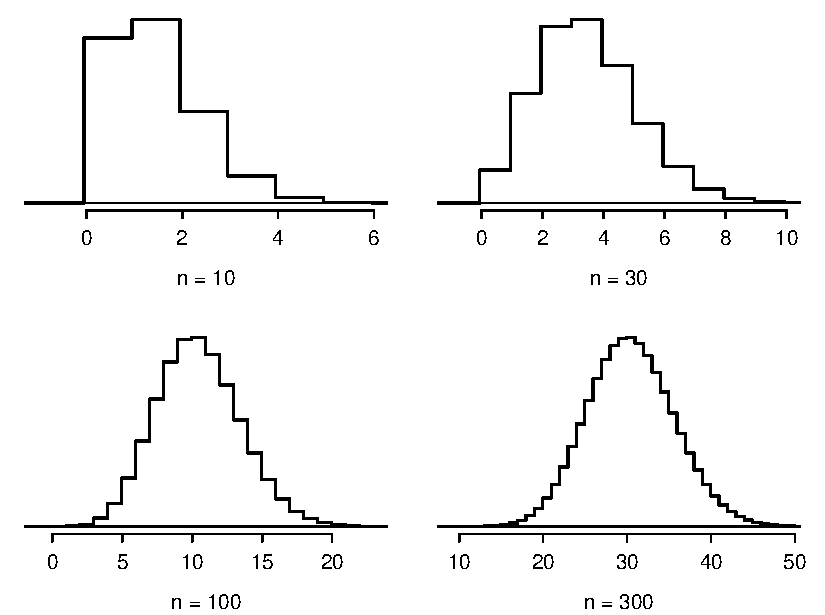
\includegraphics[width=0.60\textwidth]{4-3_binomial_distribution/figures/fourBinomialModelsShowingApproxToNormal/fourBinomialModelsShowingApproxToNormal}
\end{center}

\end{frame}

%%%%%%%%%%%%%%%%%%%%%%%%%%%%%%%%%%%

\begin{frame}
\frametitle{十分大きいとはどれくらいか？}

期待される成功回数と失敗回数がともに少なくとも10であれば、標本サイズは十分大きいと見なされる。
\[ np \ge 10 \qquad \text{かつ} \qquad n(1-p) \ge 10 \]

\soln{$10 \times 0.13 = 1.3; 10 \times (1 - 0.13) = 8.7$}

\end{frame}

%%%%%%%%%%%%%%%%%%%%%%%%%%%%%%%%%%

\begin{frame}
\frametitle{}

\pq{以下の4組の二項分布パラメータのうち、正規分布で近似できる分布はどれか？}

\begin{enumerate}[(a)]
\item $n = 100, p = 0.95$
\solnMult{$n = 25, p = 0.45$} \only<2->{\orange{$\rightarrow 25 \times 0.45 = 11.25; 25 \times 0.55 = 13.75$}}
\item $n = 150, p = 0.05$
\item $n = 500, p = 0.015$
\end{enumerate}

\end{frame}


%%%%%%%%%%%%%%%%%%%%%%%%%%%%%%%%%%%%

\begin{frame}[shrink=10]
\frametitle{Facebookユーザーの分析}

\dq{最近の研究によると「Facebookユーザーは与えるよりも多くを受け取っている」。例えば：
\begin{itemize}
\item 標本内のFacebookユーザーの40\%が友達リクエストを送ったが、63\%が少なくとも1件のリクエストを受け取った
\item ユーザーは友達のコンテンツに平均14回「いいね」を押したが、自分のコンテンツには平均20回「いいね」がついた
\item ユーザーは9件の個人メッセージを送ったが、12件を受け取った
\item ユーザーの12\%が写真で友達をタグ付けしたが、35\%が自分自身を写真でタグ付けされた
\end{itemize}
このパターンをどのように説明できるか？
}

\soln{パワーユーザーが一般ユーザーよりはるかに多くのコンテンツを投稿している。}

\ct{\webURL{http://www.pewinternet.org/Reports/2012/Facebook-users/Summary.aspx}}

\end{frame}

%%%%%%%%%%%%%%%%%%%%%%%%%%%%%%%%%%%

\begin{frame}[shrink=10]
\frametitle{}

\dq{この研究では、Facebookユーザーの約25\%がパワーユーザーと見なされることもわかった。同じ研究で、平均的なFacebookユーザーは245人の友達を持つことが明らかになった。245人の友達を持つ平均的なFacebookユーザーが、パワーユーザーと見なされる友達が70人以上いる確率は何か？必要な仮定を述べよ。}

$n = 245$、$p = 0.25$ が与えられ、確率 $P(K \ge 70)$ を求める。独立性が必要であり、ここでは仮定する（Facebookのデータにアクセスできれば確認できる）。

\begin{align*}
P(X \ge 70) &= P(K = 70\text{ または }K = 71\text{ または }\cdots\text{ または } K = 245) \\
&= P(K = 70) + P(K = 71) + \cdots + P(K = 245)
\end{align*}

これは膨大な計算になりそうだ……

\end{frame}

%%%%%%%%%%%%%%%%%%%%%%%%%%%%%%%%%%%%

\begin{frame}
\frametitle{二項分布の正規近似}

標本サイズが十分大きい場合、パラメータ $n$ と $p$ の二項分布は、パラメータ $\mu = np$、$\sigma = \sqrt{np(1-p)}$ の正規モデルで近似できる。

\begin{itemize}

\item Facebookのパワーユーザーの場合、$n = 245$、$p = 0.25$ である。
\[ \mu = 245 \times 0.25 = 61.25 \qquad \sigma = \sqrt{245 \times 0.25 \times 0.75} = 6.78 \]

\item $Bin(n = 245, p = 0.25) \approx N(\mu = 61.25, \sigma = 6.78)$。

\begin{center}
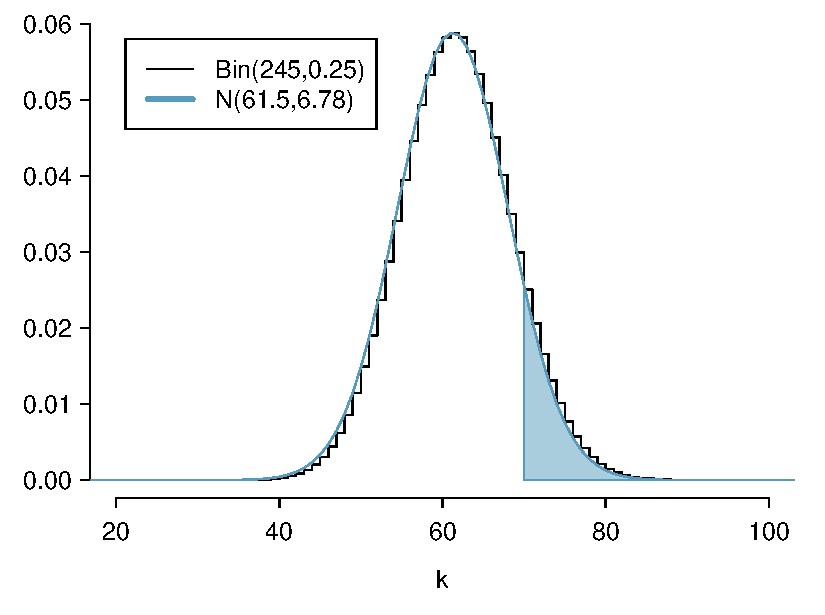
\includegraphics[width=0.5\textwidth]{4-3_binomial_distribution/figures/fb_power_user/fb_power_user}
\end{center}

\end{itemize}

\end{frame}

%%%%%%%%%%%%%%%%%%%%%%%%%%%%%%%%%%%

\begin{frame}[fragile]
\frametitle{}

\dq{245人の友達を持つ平均的なFacebookユーザーが、パワーユーザーと見なされる友達が70人以上いる確率は何か？}

\twocol{0.5}{0.5}{
\begin{center}
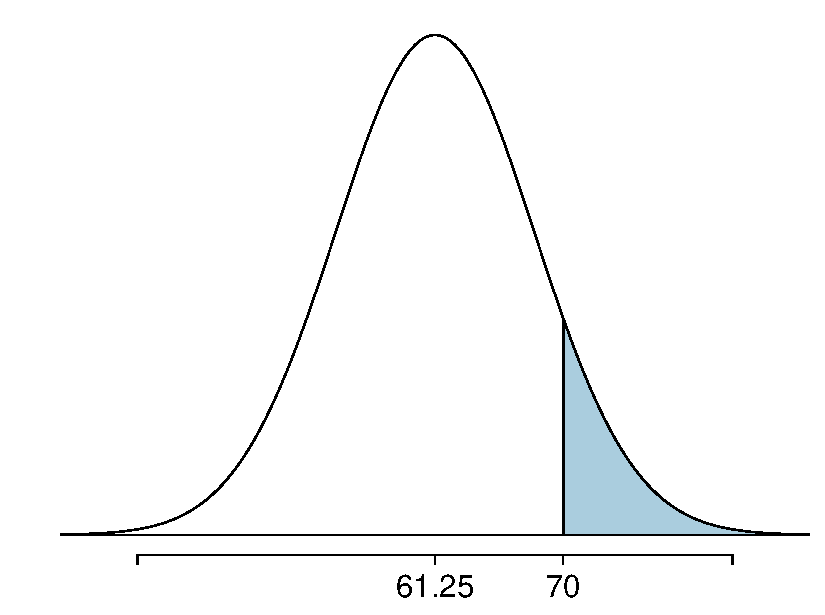
\includegraphics[width=\textwidth]{4-3_binomial_distribution/figures/fb_power_user/fb_power_user_norm}
\end{center}
}
{
{\small
\begin{align*}
Z &= \frac{\text{観測値} - \text{平均}}{SD} \\
  &= \frac{70 - 61.25}{6.78} = 1.29
\end{align*}
\[ P(Z > 1.29) = 1 - 0.9015 = 0.0985 \]
}
}

\begin{beamerboxesrounded}[shadow = true, lower = code body]{}
{\small \begin{verbatim}
> pnorm(1.29)
[1] 0.9014747
\end{verbatim}
}
\end{beamerboxesrounded}

\end{frame}

%%%%%%%%%%%%%%%%%%%%%%%%%%%%%%%%%

\subsection{小さい区間での正規近似の限界}

%%%%%%%%%%%%%%%%%%%%%%%%%%%%%%%%%%%%

\begin{frame}
\frametitle{小さい区間での正規近似の限界}

\begin{itemize}

\item 二項分布に対する正規近似は、条件が満たされていても、少数の値の範囲の確率を推定する際に精度が低下する傾向がある。

\item 値の区間に対するこの近似は、カットオフ値を両方向に0.5ずつ拡張することで通常改善される。

\item 正規近似を適用する際にこの修正を加えるヒントは、観測値の範囲を調べる際に最も役立つ。裾確率を計算する際にもこの修正を適用することは可能だが、区間が通常かなり広いため修正の利点は消えることが多い。

\end{itemize}

\end{frame}

%%%%%%%%%%%%%%%%%%%%%%%%%%%%%%%%%%%
